\documentclass[tikz, border=10pt]{standalone}
\usepackage{tikz}
\usetikzlibrary{calc, angles, quotes}

\begin{document}
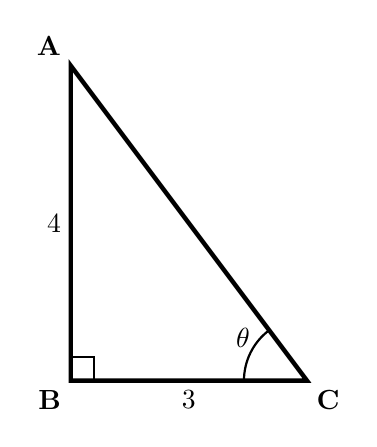
\begin{tikzpicture}

% Define vertices
\coordinate (A) at (0, 4);
\coordinate (B) at (0, 0);
\coordinate (C) at (3, 0);

% Draw the triangle
\draw[ultra thick] (A) -- (B) -- (C) -- cycle;

% Right angle mark at B
\def\sq{0.3}
\draw[thick] (B) ++(0, \sq) -- ++(\sq, 0) -- ++(0, -\sq);

% Angle theta at C
\draw[thick] ($(C)+(-0.8, 0)$) arc (180:127:0.8);
\node[above left, font=\normalsize] at ($(C)+(-0.6, 0.3)$) {$\theta$};

% Labels for vertices
\node[above left] at (A) {\textbf{A}};
\node[below left] at (B) {\textbf{B}};
\node[below right] at (C) {\textbf{C}};

% Dimension label: AB = 4 (left side)
\node[left, font=\normalsize] at ($(A)!0.5!(B)$) {4};

% Dimension label: BC = 3 (bottom side)
\node[below, font=\normalsize] at ($(B)!0.5!(C)$) {3};

\end{tikzpicture}
\end{document}